% !TeX root = ../dissertation.tex

\section{Evaluation}
\label{sec:trilliumeval}

% \begin{figure*}[!ht!!]
% 	\centering
% 	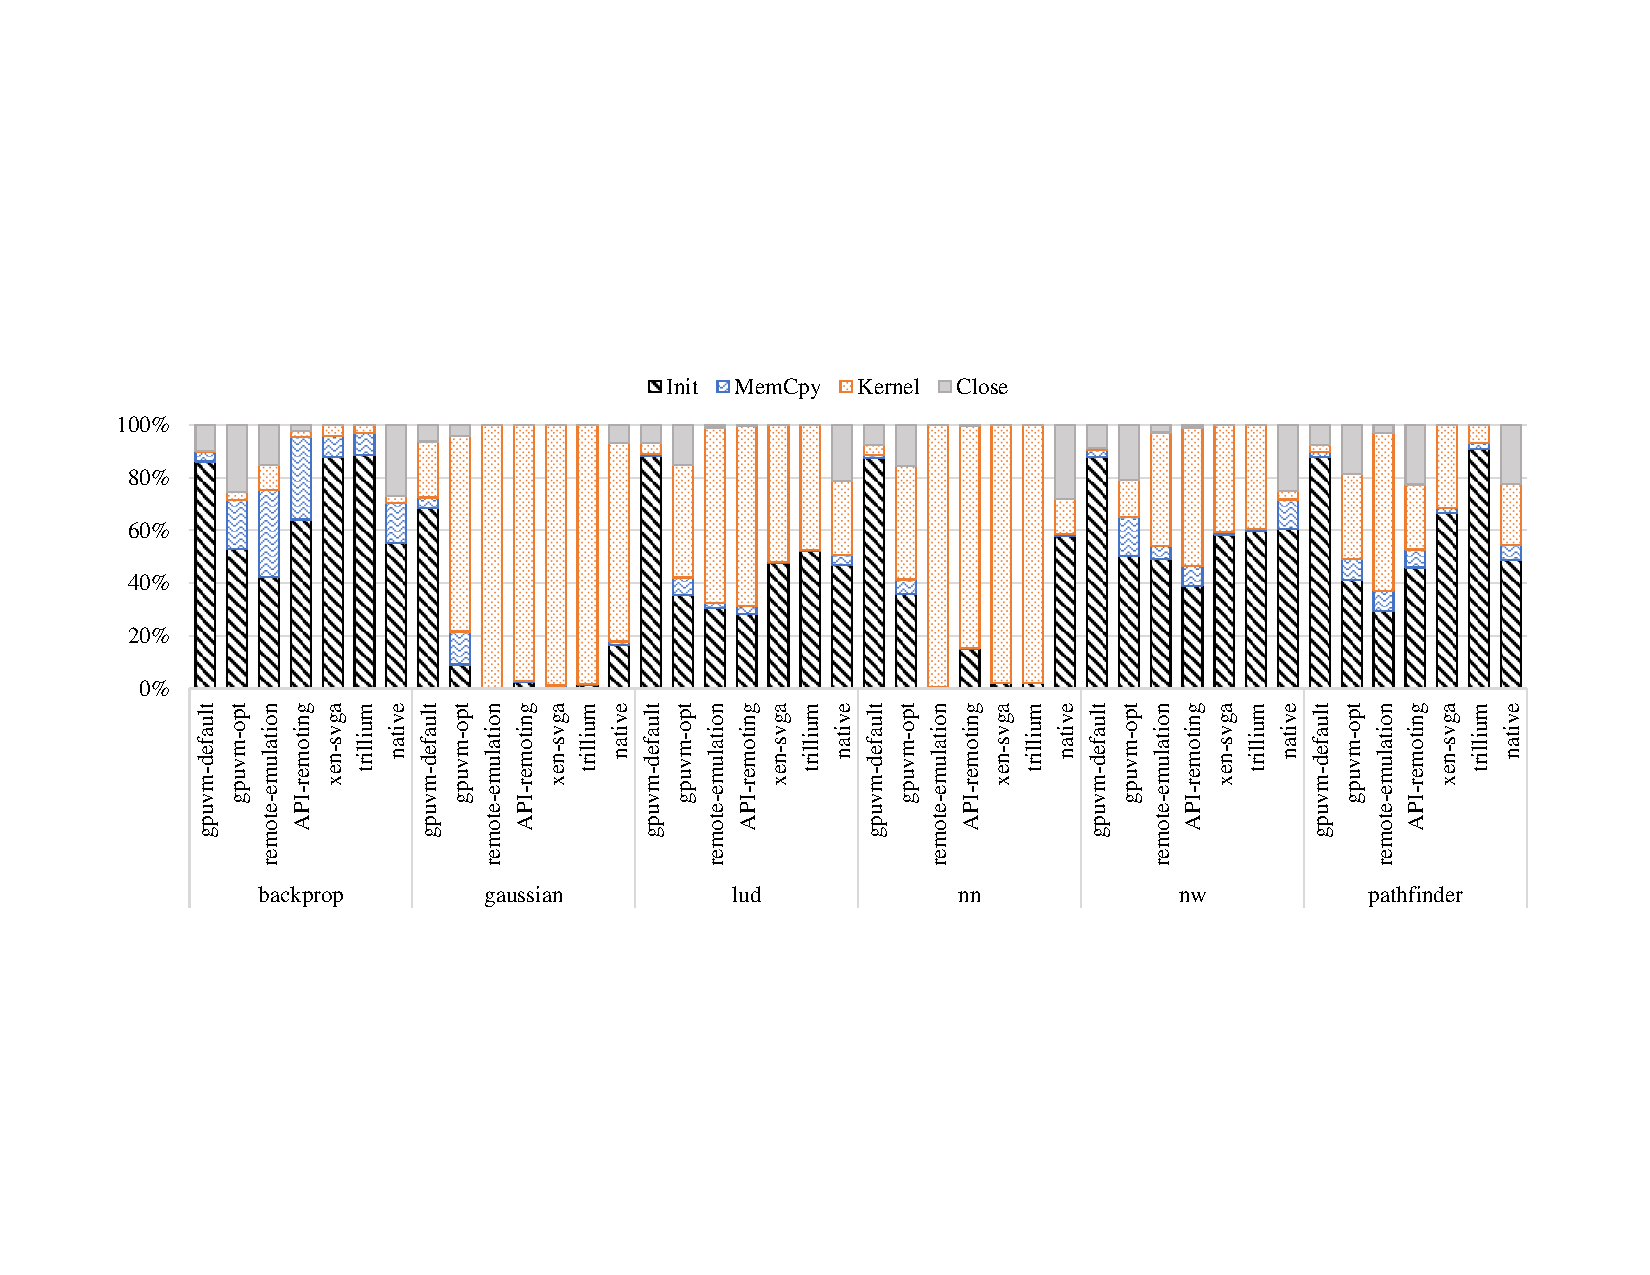
\includegraphics[width=.9\linewidth,trim={2cm 6cm 2cm 6cm},clip]{data/cross_product_breakdown_noRPC_OptInit.pdf}
% 	\caption{{\footnotesize Runtime breakdown of GPU benchmarks on virtualization prototypes.}}
% 	\label{fig_all_breakdown} \end{figure*}

We are interested in understanding the impact of a vISA on end-to-end performance, the effect of interposition frequency on performance, and the effectiveness of our proposed design, \Trillium.

\subsection{The impact of vISA choice}

%% \begin{figure}[!ht]
%% 	\centering
%% 	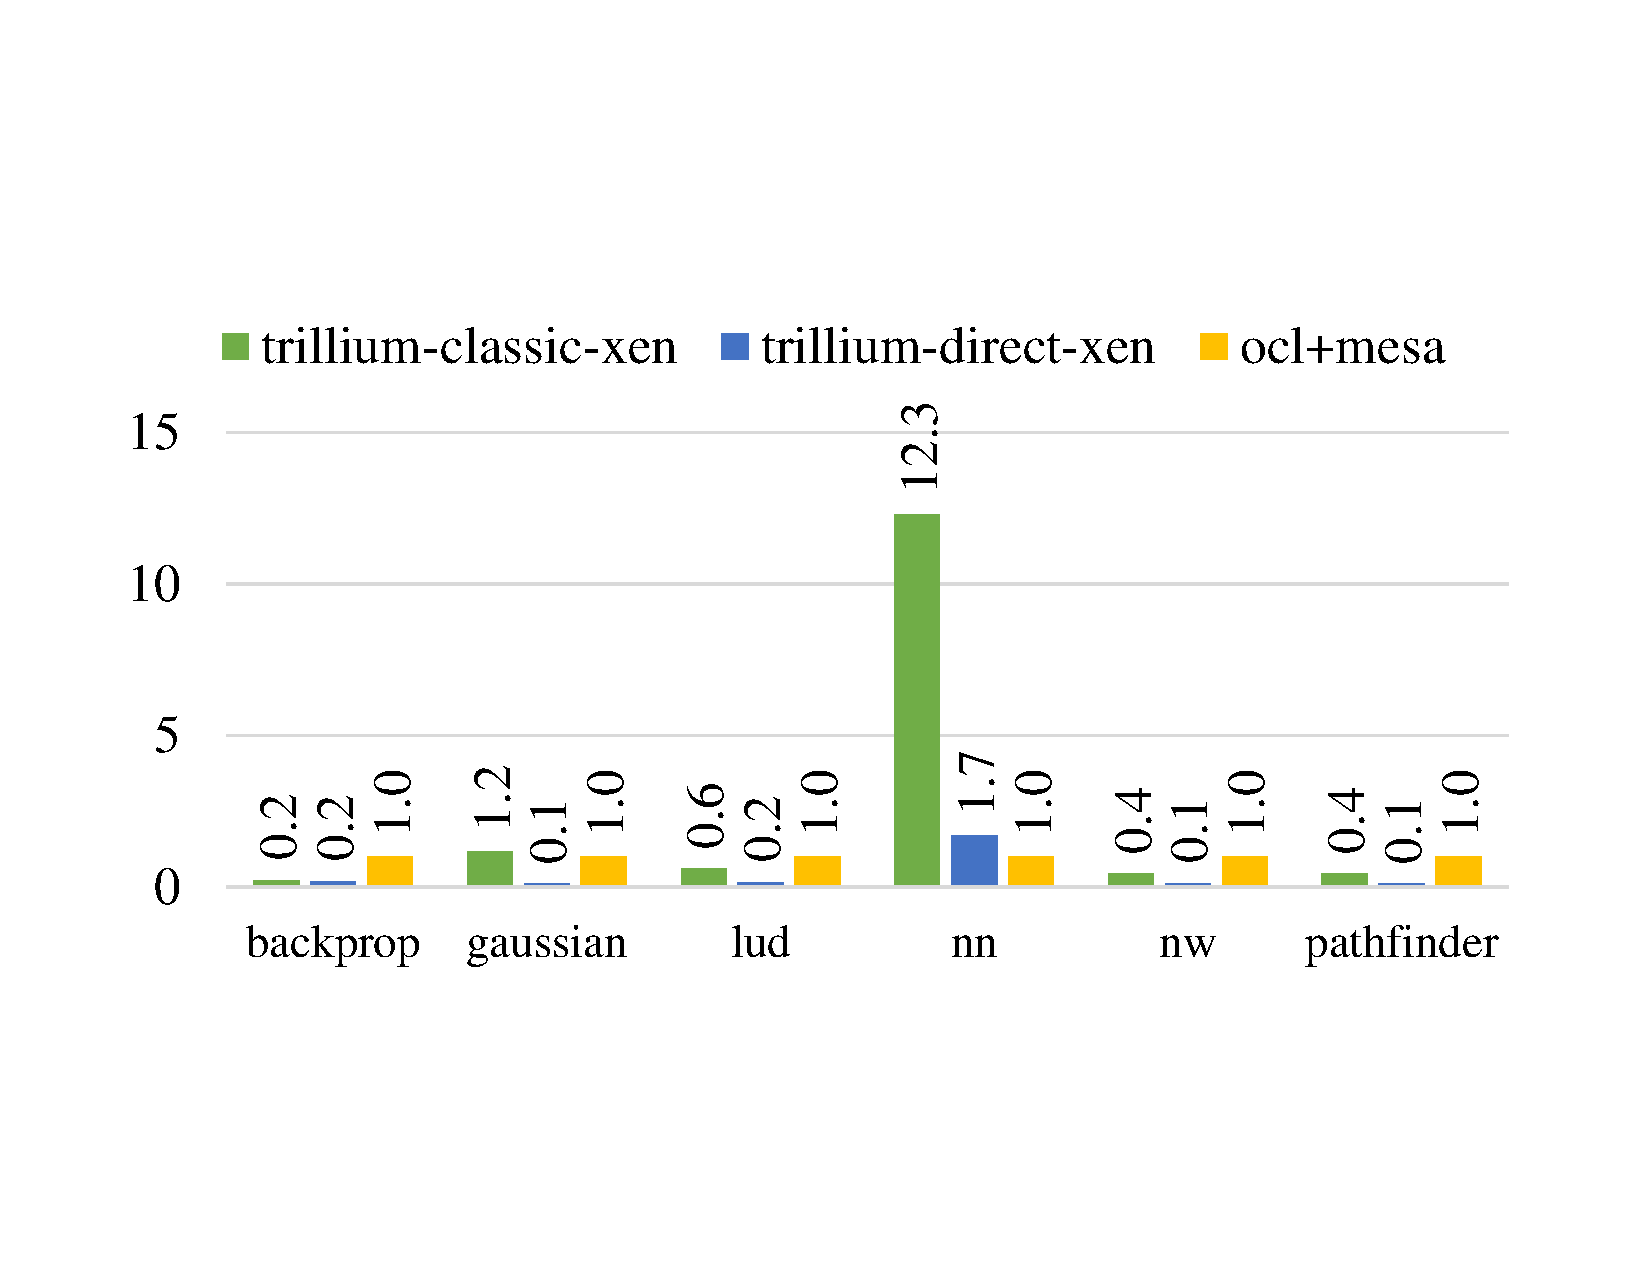
\includegraphics[width=\linewidth,trim={2.2cm 5cm 2.2cm 5.5cm},clip]{data/trillium/pipe_overhead_noRPC_OptInit.pdf}
%% 	\caption{{\footnotesize Overheads of the Trillium models with shadow pipe. \texttt{OpenCL+Mesa} is the baseline.}}
%% 	\label{fig_pipe_overhead} \end{figure}

%% \begin{figure}[!ht]
%% 	\centering
%% 	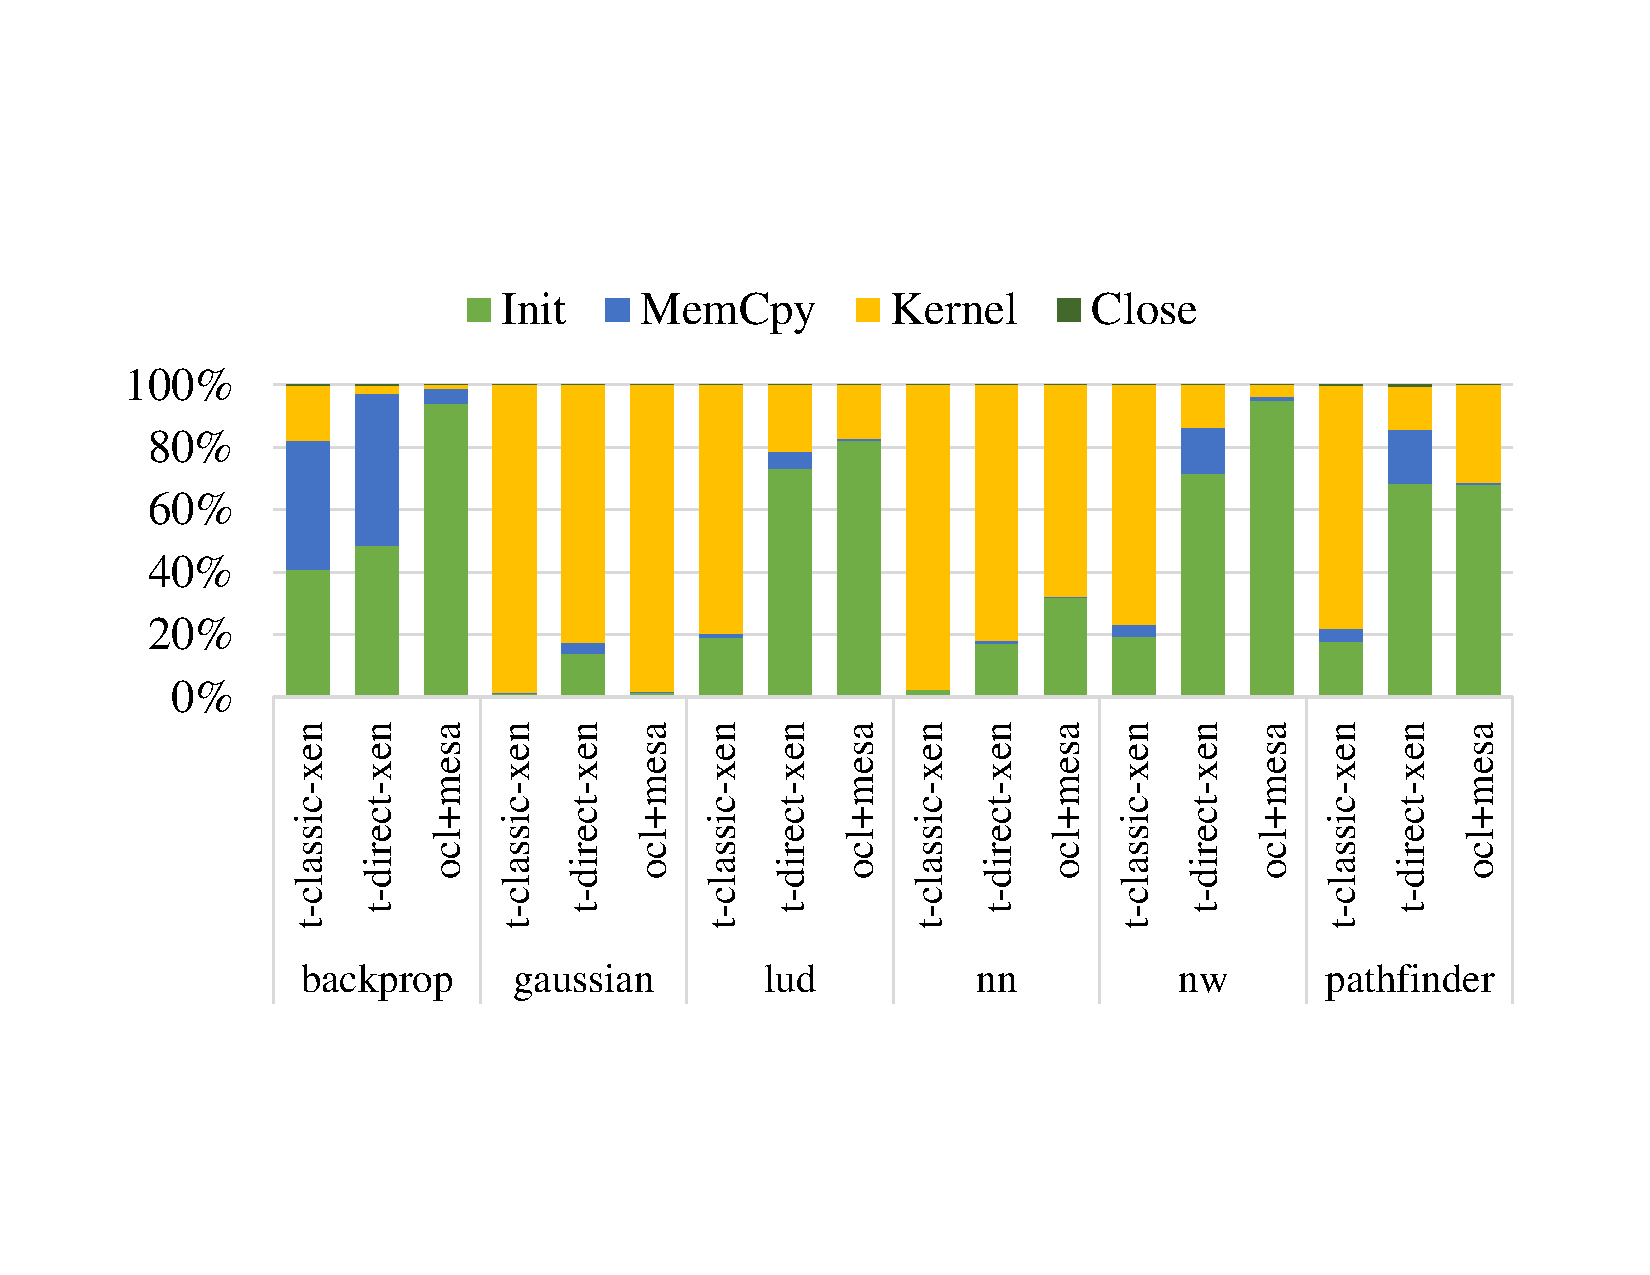
\includegraphics[width=\linewidth,trim={2.2cm 4.5cm 2.2cm 4.8cm},clip]{data/trillium/pipe_breakdown_noRPC_OptInit.pdf}
%% 	\caption{{\footnotesize Rumtime breakdown of the GPU benchmarks on the Trillium models with shadow pipe.}}
%% 	\label{fig_pipe_breakdown} \end{figure}

% The key difference between \Trillium-classic and \Trillium-direct is
% avoiding the use of a virtual instruction set in the guest.
% This eliminates a compiler transformation, but more importantly
% impacts
% these effects are visible, to put them in starker relief,
% the vendor-supplied compiler to be used under the virtualization layer
% (in this case the NVIDIA OpenCL stack), and for a design that produces
% LLVM in the guest, and finalizes that to NVIDIA SASS in the hypervisor.

%We re-iterate that our TGSI implementation is unoptimized
%and quantifying the performance loss attributable to that alone is difficult.

% \aak {I'm tempted to just remove the following. It doesn't really add anything to the paper.}
% We manually inspected the SASS binaries produced by the Nvidia and open source
% frameworks to understand the performance differences. While an in depth of
% analysis is beyond the scope of this paper, we make the following observations.

% \begin{compactitem}
% \item Both of the binaries benefit from common optimizations such as loop
% 	unrolling, and constant propagation, courtesy of LLVM.
% \item SASS code produced through the TGSI has substantially more convergence
% 	points (SYNC and SSY) instructions, which represent additional opportunity
% 	for control flow divergence.
% 	 % Table~\ref{tab:sassdiferences} presents the number of control flow instructions in the two binaries, as a proxy for diverging control flow.
% \item NVIDIA-produced SASS produces very different instruction sequences in
% 	several cases, e.g. XMAD (16bit Multiply Add) vs FFMA in TGSI (32-bit
% 	Fused Multipy Add). Our conjecture, in keeping with our hypothesis, is
% 	that the NVIDIA compiler has better information about which instructions
% 	more efficent on a particular architecture. It may be possible to
% 	reproduce some of these optimizations in the TGSI to SASS transformation,
% 	but since production of the TGSI code cannot rely on knowledge of the
% 	architecture, some optimizations may be impossible.
% \end{compactitem}
% \cjr{update me Amogh!}
% % !TeX root = ../dissertation.tex
\begin{table*}[h!]
\centering
% \footnotesize{
\begin{tabular}{@{}lllllllll@{}}
\toprule
           & \multicolumn{4}{l}{LLVM+PTXAS} & \multicolumn{4}{l}{Clover+Nouveua} \\ \midrule
           & SYNC    & SSY   & BRA   & BB   & SYNC     & SSY    & BRA    & BB    \\
bfs        & 0       & 0     & 15    & 12   & 8        & 4      & 5      & 18    \\
gaussian   & 0       & 0     & 23    & 18   & 6        & 3      & 3      & 9     \\
nn         & 0       & 0     & 9     & 7    & 0        & 0      & 0      & 4     \\
nw         & 10      & 5     & 18    & 23   & 8        & 4      & 8      & 18    \\
pathfinder & 9       & 5     & 18    & 23   & 12       & 6      & 7      & 32    \\
lud        & 31      & 13    & 67    & 76   & 20       & 10     & 14     & 35    \\ \bottomrule
\end{tabular}
% }
\caption{\footnotesize{Possible sources of performance differences between kernels generated using LLVM+PTXAS (comparable to NVCC) and Clover+Nouveau.}}
\label{tab:sassdiferences}
\end{table*}

% Table~\ref{tb_clover_slowdown} shows slowdowns of the Clover OpenCL runtime.\cjr{what is this  supposed to be?}
% \hyu{We wanted to factor out the impact of runtime. This table is not useful if we don't need to analyze the performance
% of Clover. It seems that we are only focusing on the Kernel time.}


\begin{figure*}[!ht!!]
	\centering
	% \includegraphics[width=.9\linewidth,trim={2cm 7.5cm 2cm 7cm},clip]{data/cross_product_overhead_noRPC_OptInit.pdf}
	\includegraphics[width=.9\linewidth,clip]{trillium/data/cross_product_overhead_noRPC_OptInit.pdf}
	\caption{{\footnotesize End-to-end execution times of benchmarks on virtualization prototypes, relative to end-to-end execution time on the NVIDIA CUDA runtime in a native setting.
			The gRPC transport overhead is removed from the reported measurements, which is up to 10\% of the total execution time for API remoting, and 40\% for \Trillium.}}
	\label{fig_all_overhead} \end{figure*}

\begin{figure}[!ht]
	\centering
	% ,trim={2.2cm 5cm 2.2cm 5.5cm},clip
	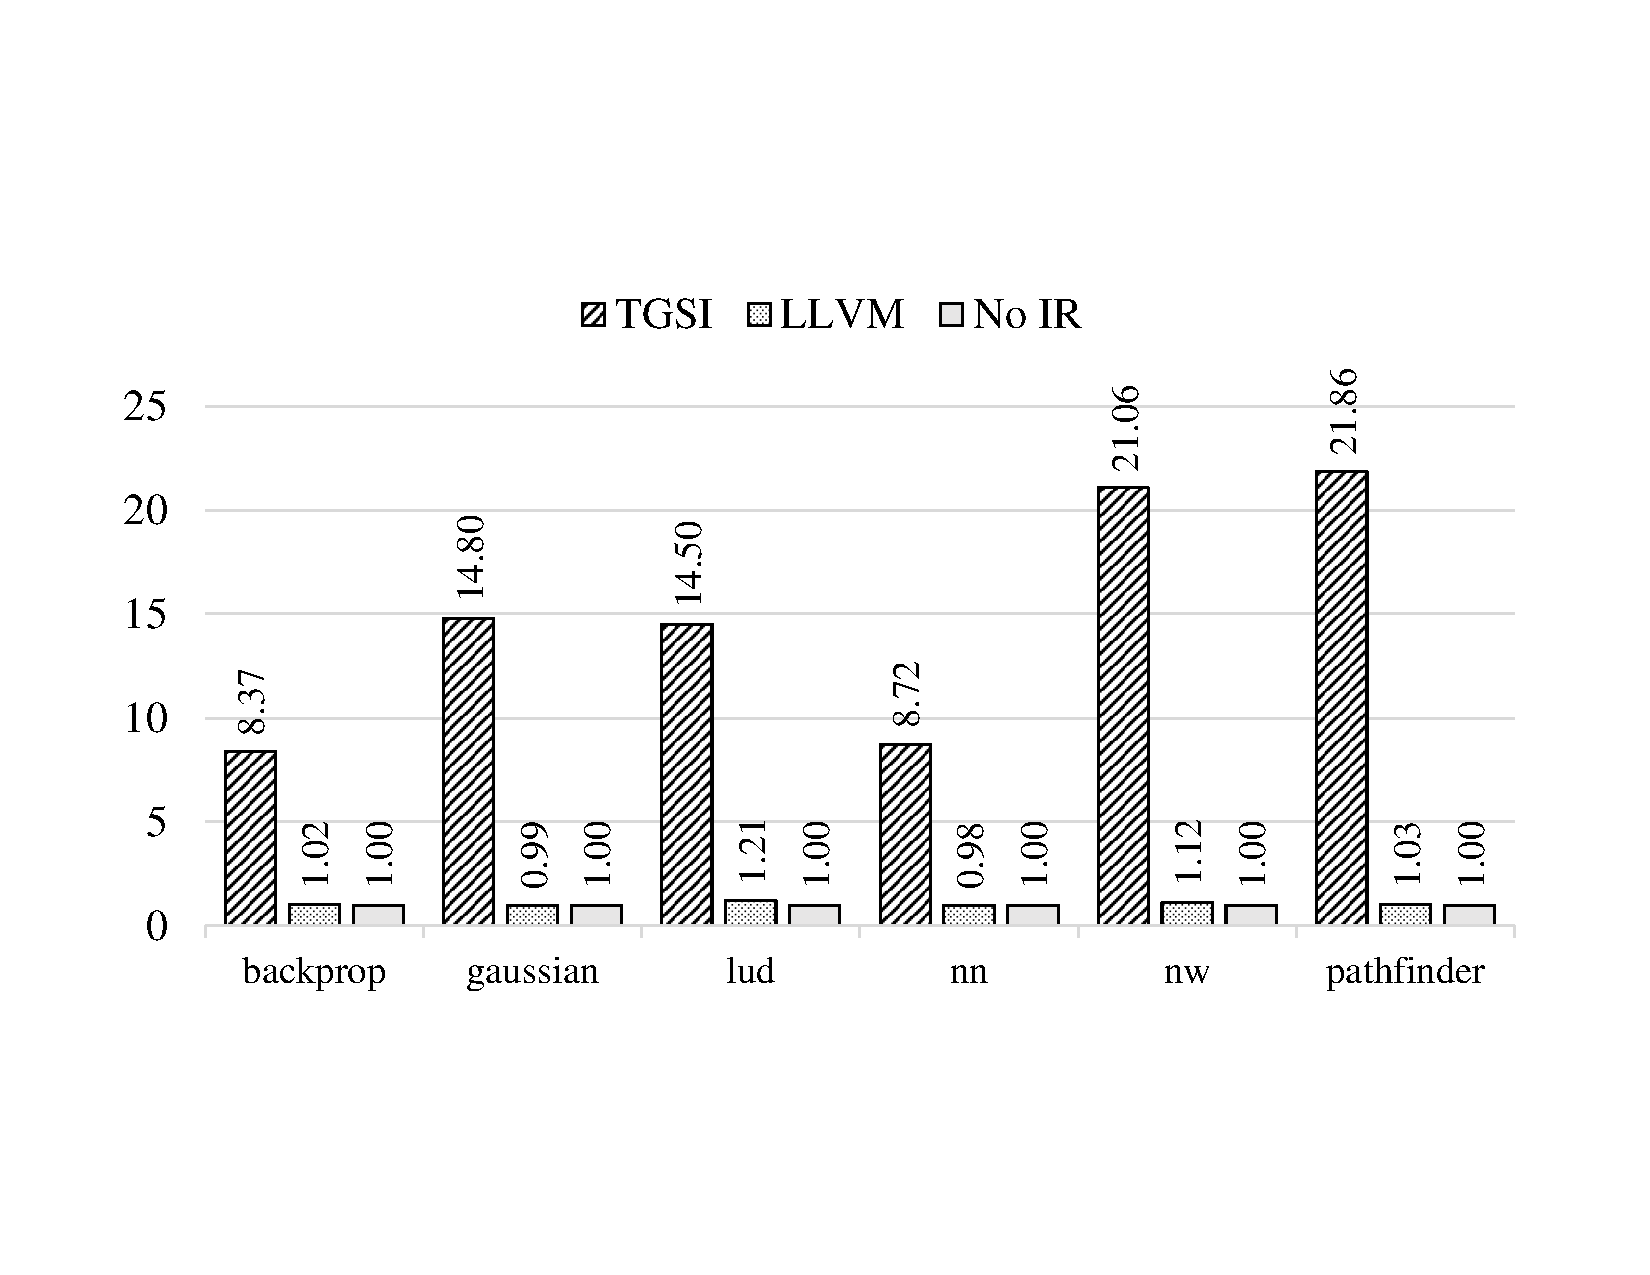
\includegraphics[width=.9\linewidth,trim={2cm 4.5cm 2cm 5cm},clip]{trillium/data/trillium/trillium_kernel.pdf}
	\caption{{\footnotesize Kernel execution slowdown due to virtual ISAs. TGSI: the LLVM TGSI back-end compiler used in \XenSVGA. LLVM: LLVM NVIDIA PTX (NVPTX) back-end used in \Trillium. No IR: native NVIDIA compiler.}}
	\label{fig_trillium_kernel}
\end{figure}

Deferring the compilation of front-end code to the host not only
eliminates redundant translations, and the need to have a compiler in the
guest driver,
 % that can translate supported compute frameworks to TGSI,
but also ensures that the compiler has a high-fidelity view of
the physical hardware. Typically, the execution/compilation framework is
extremely tightly coupled with the vISA used, making the choice of vISA even
more tenuous as it leads to the second order effect of having to rely on a
particular implementation of the compute framework (e.g., Mesa3D OpenCL vs NVIDIA OpenCL).
% This is especially significant given the nature of GPGPU computation.
%, instead ofhaving the option to use the best performing framework.

To understand the impact of the virtual ISA on the quality of the generated GPU code
% code that is ultimately run on the hardware,
we measured GPU execution time for NVIDIA SASS kernels generated in 3 ways:
a) using the Mesa3d OpenCL stack (OpenCL$\rightarrow{}$TGSI$\rightarrow{}$SASS),
b) using the LLVM OpenCL stack (OpenCL$\rightarrow{}$LLVM IR$\rightarrow{}$SASS),
and c) using the native NVIDIA OpenCL compiler (OpenCL$\rightarrow{}$SASS).
% , leaving out other overheads
% induced for virtualization, data, and device management.
These measurements are reported in Figure~\ref{fig_trillium_kernel}
relative to kernel execution time in a native setting.
% The Mesa3D OpenCL stack (Clover$+$Nouveau), which uses the TGSI
% ISA internally, is used to examine \XenSVGA and \Trillium.
%and by executing OpenCL code natively using the NVIDIA OpenCL framework.
%We were unable to to separate the execution/compilation framework
%from the ISA used, due their extremely tight coupling.


Code generated from TGSI IR is dramatically slower in all cases than code
generated by the NVIDIA OpenCL framework. We observe slowdowns of up to 22$
\times$, with a harmonic mean of 13$\times$ across the 6 benchmarks that were
optimized for evaluation.
% \hyu{Mention why pick 6?}
While we
predicted the basic trend these experiments show, we were surprised by the
magnitude of the difference. We found quality of the kernel generated by the
LLVM NVPTX compiler to be comparable to native, at least in terms of execution
time. This is unsurprising given recent efforts~\cite{gpucc} to optimize the
LLVM tool-chain for NVIDIA GPUs.

The \Trillium design uses LLVM IR as the common virtual ISA for GPGPU applications,
where necessary: OpenCL code is compiled to PTX using the LLVM NVPTX back-end in the guest,
and then finalized and executed in the host using the NVIDIA CUDA framework.

% SPIR-V has recently been adopted by the MESA3D community as an alternative to
% TGSI. SPIR-V is designed explicitly for expressing GPGPU primitives, and thus is likely
% to display better performance. However, our core conclusion still applies:
% vISAs introduced by the graphics stack are an unnecessary translation layer.

%(Control experiments show that choice of compute framework has negligible
%impact on the kernel execution time. See Section~\ref{sec:control})
% The data suggests that LLVM IR may be a suitable vISA as it enables GPU code
% whose quality is not substantially different from native execution.

\subsection{End-to-End}


We compare \Trillium against full-virtual (\gpuvmdef and \gpuvmopt),
API remoting (\apigpu and \apicpu) and para-virtual (\XenSVGA) systems.
\XenSVGA approximates an SVGA-like design in Xen (Mesa3D with TGSI). \Trillium
% is very similar, other than that it
bypasses translation from OpenCL to TGSI.
To characterize the behavior a full-virtual\-ization design, we measure
GPUvm~\cite{GPUvm} in its default configuration (worst case) shown as \gpuvmdef,
and in its fully optimized configuration, labeled \gpuvmopt.
% We additionally API remoting, both with GPU and CPU back-end.

%\aak{We need to reword this claim, because we aren't the closest to native performance. That claim sits firmly with api-remoting. However, we do much better than api-remoting on other aspects, and are thus a more complete virtualization mechanism in some sense.}
%\cjr{dispatched.}
% \hyu{Good point.}
% \aak{Also, we need to explain why we ran only 6 applications, given that we claimed that 10 benchmarks could be built by the compiler (in the implementation section. The reduction in number is because of the effort of porting applications to work on the API-forwarding we used to implement Trillium. We have to explain that.)}
% \hyu{Explanations in my head: 1. space limit; 2. these 6 are representitive. Strong enough?}
% \cjr{Not sure I'd buy space limit as the argument. Plus it's not really true right?}

Figure~\ref{fig_all_overhead} shows the end-to-end execution time (relative to
native GPU execution) for the six chosen benchmarks for all the systems evaluated. As
expected, traditional API remoting designs incur the lowest overhead, which is
achieved by giving up hypervisor interposition.
\Trillium fares well with best case performance
of just 1.1$\times$ over native, and within 3.6$\times$ at worst. \XenSVGA is
sensitive to the performance lost in GPU kernel code resulting from redundant
compilation through TGSI (which adds significant overheads as previously shown in
Figure~\ref{fig_trillium_kernel}). \gpuvmopt exhibits about 9.1$\times$ slowdown for
applications with short-lived kernels (e.g. Needleman-Wunsh algorithm); the
overhead can be as high as 15.2$\times$ when the workload has long-running
kernels (e.g. Gaussian Elimination).
% \hyu{May be good to analyze D/R/M categories' performance.}
% \aak{Agreed, but there doesn't seemt to be any correlation between D/R/M and Trillium's performance. I don't understand why the behaviour exhinbited is the way it is, and at this point, meh.}

We find that remoting calls intended to a CPU is uniformly more
performant than full-virtualization of the GPU, and sometimes performs just as well as (backprop)
or better than remoting to the GPU (1.6$\times$ faster for the bfs benchmark. The performance gain
from accelerating the bfs kernel on the GPU is severely dwarfed by the cost of initialization on
the GPU).
% \hyu{Analyze the reason? Maybe quote some part of Section VI-A?}
% \aak{Again I don't really have the patience go dig it up... Let's make sure we understand our data really well for Ava... This conference is meh as it is...}
% We do not suggest that GPGPU virtualization designers should use CPUs; instead,
% We make two observations about this situation:
GPGPU compute is only economical when it provides acceleration over the CPU;
if overheads make the CPU competitive, the profitability threshold has been crossed.
Further, the competitiveness of \apicpu suggests opportunity: systems could back a virtual
GPU with CPU if they can detect when it is profitable to do so.

% Application types can impact performance greatly.
% Note that for GPUvm, GPU kernel execution time did not differ significantly from other systems before ported to newer Ubuntu and Xen platform;
% The dramatic overheads on GPUvm are mostly attributable to the use of trap-based interposition on communication through memory-mapped command queues and/or MMIO.
%\XenSVGA delivers similar performance in general to the best-case full virtualization system.

% \subsection{Runtime Breakdown} \label{sec:breakdown}

% Benchmark applications operate in several different phases:
% initialization, data transfer, GPU kernel execution, and close/ teardown, each of responds differently to the different virtualization mechanisms. To illustrate this, we present the percentage of time spent in initialization, data transfer, GPU kernel execution, and close/teardown for each benchmark and system in Figure~\ref{fig_all_breakdown}.
% \aak{What is the point we're trying to make here? Too tired...}
% As noted earlier, the benchmarks can be classified into three categories: \textit{interposition-dominant} benchmarks (e.g. gaussian and nn) that see lower overheads from \Trillium
% \textit{interposition-rare} applications (e.g. backprop and pathfinder) which run a small number of long-running kernels, thereby suffering very little API-interposition overhead, and additionally benefit from the speedup in \texttt{Init} time (pre-initialized by remote server).
% \textit{moderate-interposition} applications (e.g. lud, nw) which invoke a
% moderate number of API calls, and therefore bear some interposition induced
% overhead.
% For interposition-dominant benchmarks, \XenSVGA performs really poorly because of the . \Trillium is efficient because that layer is bypassed and interposed APIs are batched.

% \subsection{Miscellanea}

%% \subsection{API remoting}

%% The major overheads of API remoting method are caused by RPC and data transfer. We applied widely-used Google
%% Protocol Buffers and XML-RPC to implement the RPC client (the one which runs the benchmarks) and server
%% (the one which actually executes the GPU commands). However, data transfer can be accomplished using shared memory rings~\cite{xen}
%% or remote direct memory access (RDMA), dramatically lowering these costs relative to our prototype.~\cjr{check this later. are we reporting these overheads?}
%% \hyu{We report the RPC time, but exclude the data transfer time.}
%% \hyu{The data makes less sense if we also exculde the RPC time; then there'll be trivial overheads. But our current RPC implementation is too naive, leading to non-trivial RPC overheads; this fails our trillium-pipe to outperform GPUvm-opt.}
%% \hyu{The best case is where we have an excellent RPC framework.}
%% \hyu{Data used to exclude trillium-classic-xen's RPC time: data/trillium/pipe.xlsx . We aren't able to exclude
%% 	the RPC overhead of trillium-direct-xen because we don't have a really running prototype.}


%% RPC number Table~\ref{tb:rpc_num}. \hyu{this table seems helpful.}

%% \begin{comment}
%% \begin{table*}[!th]
%% 	\centering
%% 	\begin{tabular}{l|r|r|r|r|r|r|}
%% 		\cline{2-7}
%% 		& \multicolumn{1}{l|}{backprop} & \multicolumn{1}{l|}{gaussian} & \multicolumn{1}{l|}{lud} & \multicolumn{1}{l|}{nn} & \multicolumn{1}{l|}{nw} & \multicolumn{1}{l|}{pathfinder} \\ \hline
%% 		\multicolumn{1}{|l|}{api-remoting} & 46 & 12,298 & 2,688 & 2,018 & 552 & 91 \\ \hline
%% 		\multicolumn{1}{|l|}{shadow-pipe} & 33 & 22,514 & 4,208 & 11,007 & 2,813 & 66 \\ \hline
%% 	\end{tabular}
%% 	\caption{\footnotesize{Number of RPCs sent in API remoting and Trillium models.}}
%% 	\label{tb:rpc_num}
%% \end{table*}

%% RPC overhead Table~\ref{tb:rpc_overhead_abs} and \ref{tb:rpc_overhead_relative} \hyu{may confuse the reader. RPC overhead
%% 	depends on the RPC number, RPC size, and RPC cost percentage also depends on the end-to-end time. E.g. RPC takes much higher portion in api-remoting gaussian and nn, because the kernel time is much shorter, and frequent clSetKernelArg API calls are
%% 	required.}
%% \begin{table*}[]
%% 	\centering
%% 	\begin{tabular}{l|r|r|r|r|r|r|}
%% 		\cline{2-7}
%% 		& \multicolumn{1}{l|}{backprop} & \multicolumn{1}{l|}{gaussian} & \multicolumn{1}{l|}{lud} & \multicolumn{1}{l|}{nn} & \multicolumn{1}{l|}{nw} & \multicolumn{1}{l|}{pathfinder} \\ \hline
%% 		\multicolumn{1}{|l|}{api-remoting} & 24.68 & 3,908.87 & 232.12 & 715.03 & 278.55 & 30.18 \\ \hline
%% 		\multicolumn{1}{|l|}{shadow-pipe} & 17.42 & 10812.96 & 2338.37 & 5319.76 & 1319.14 & 26.46 \\ \hline
%% 	\end{tabular}
%% 	\caption{\footnotesize{RPC overheads in API remoting and Trillium models (milliseconds)}}
%% 	\label{tb:rpc_overhead_abs}
%% \end{table*}

%% \begin{table*}[]
%% 	\centering
%% 	\begin{tabular}{l|r|r|r|r|r|r|}
%% 		\cline{2-7}
%% 		& \multicolumn{1}{l|}{backprop} & \multicolumn{1}{l|}{gaussian} & \multicolumn{1}{l|}{lud} & \multicolumn{1}{l|}{nn} & \multicolumn{1}{l|}{nw} & \multicolumn{1}{l|}{pathfinder} \\ \hline
%% 		\multicolumn{1}{|l|}{api-remoting} & 2.79\% & 81.20\% & 30.14\% & 77.97\% & 37.18\% & 5.25\% \\ \hline
%% 		\multicolumn{1}{|l|}{shadow-pipe} & 0.56\% & 58.92\% & 26.92\% & 57.33\% & 22.13\% & 0.64\% \\ \hline
%% 	\end{tabular}
%% 	\caption{\footnotesize{Percentages of the RPC cost in API remoting and Trillium models.}}
%% 	\label{tb:rpc_overhead_relative}
%% \end{table*}
%% \end{comment}
